\paragraph{Question 2.1}
Ci-dessous le graphe correspondant \`a l'exemple propos\'e.
\begin{figure*}[h]
\centering
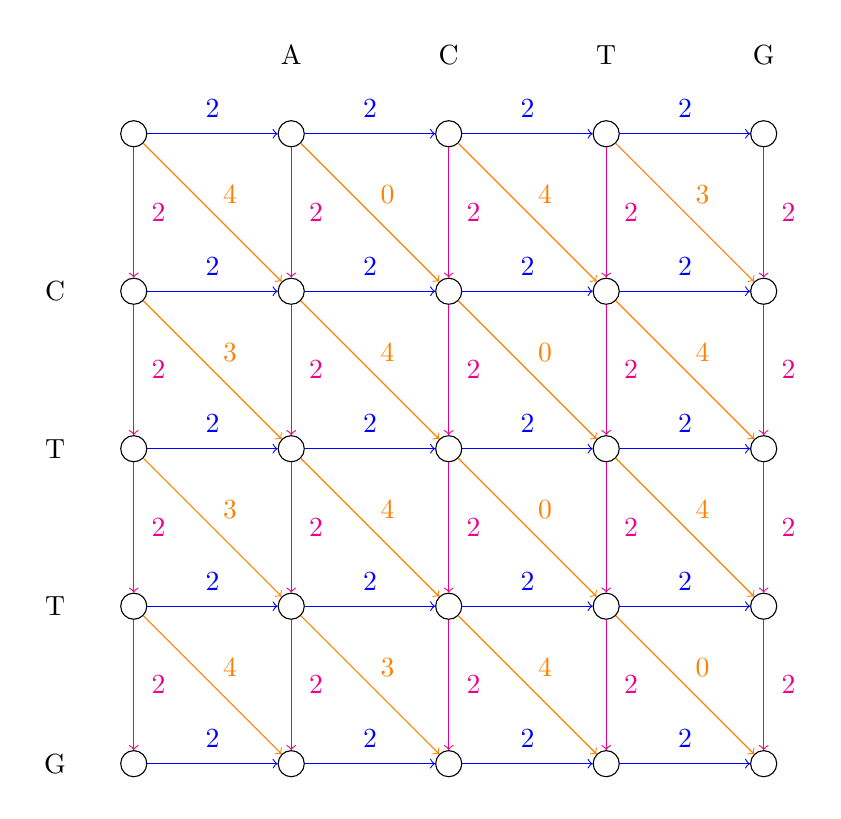
\begin{tikzpicture}[shape=circle,auto]
    \node[draw] (A) at (0,0) {};
    \node[draw] (B) at (2,0) {};
    \node[draw] (C) at (4,0) {};
    \node[draw] (D) at (6,0) {};
    \node[draw] (E) at (8,0) {};
    \node[draw] (F) at (0,2) {};
    \node[draw] (G) at (2,2) {};
    \node[draw] (H) at (4,2) {};
    \node[draw] (I) at (6,2) {};
    \node[draw] (J) at (8,2) {};
    \node[draw] (K) at (0,4) {};
    \node[draw] (L) at (2,4) {};
    \node[draw] (M) at (4,4) {};
    \node[draw] (N) at (6,4) {};
    \node[draw] (O) at (8,4) {};
    \node[draw] (P) at (0,6) {};
    \node[draw] (Q) at (2,6) {};
    \node[draw] (R) at (4,6) {};
    \node[draw] (S) at (6,6) {};
    \node[draw] (T) at (8,6) {};
    \node[draw] (U) at (0,8) {};
    \node[draw] (V) at (2,8) {};
    \node[draw] (W) at (4,8) {};
    \node[draw] (X) at (6,8) {};
    \node[draw] (Y) at (8,8) {};
    
    \draw (2,9) node{A};
    \draw (4,9) node{C};
    \draw (6,9) node{T};
    \draw (8,9) node{G};
    \draw (-1,0) node{G};
    \draw (-1,2) node{T};
    \draw (-1,4) node{T};
    \draw (-1,6) node{C};

    \draw (A) edge[blue, ->] node {2} (B);
    \draw (B) edge[blue, ->] node {2} (C);
    \draw (C) edge[blue, ->] node {2} (D);
    \draw (D) edge[blue, ->] node {2} (E);
    \draw (F) edge[blue, ->] node {2} (G);
    \draw (G) edge[blue, ->] node {2} (H);
    \draw (H) edge[blue, ->] node {2} (I);
    \draw (I) edge[blue, ->] node {2} (J);
    \draw (K) edge[blue, ->] node {2} (L);
    \draw (L) edge[blue, ->] node {2} (M);
    \draw (M) edge[blue, ->] node {2} (N);
    \draw (N) edge[blue, ->] node {2} (O);
    \draw (P) edge[blue, ->] node {2} (Q);
    \draw (Q) edge[blue, ->] node {2} (R);
    \draw (R) edge[blue, ->] node {2} (S);
    \draw (S) edge[blue, ->] node {2} (T);
    \draw (U) edge[blue, ->] node {2} (V);
    \draw (V) edge[blue, ->] node {2} (W);
    \draw (W) edge[blue, ->] node {2} (X);
    \draw (X) edge[blue, ->] node {2} (Y);

    \draw (F) edge[magenta, ->] node {2} (A);
    \draw (G) edge[magenta, ->] node {2} (B);
    \draw (H) edge[magenta, ->] node {2} (C);
    \draw (I) edge[magenta, ->] node {2} (D);
    \draw (J) edge[magenta, ->] node {2} (E);
    \draw (K) edge[magenta, ->] node {2} (F);
    \draw (L) edge[magenta, ->] node {2} (G);
    \draw (M) edge[magenta, ->] node {2} (H);
    \draw (N) edge[magenta, ->] node {2} (I);
    \draw (O) edge[magenta, ->] node {2} (J);
    \draw (P) edge[magenta, ->] node {2} (K);
    \draw (Q) edge[magenta, ->] node {2} (L);
    \draw (R) edge[magenta, ->] node {2} (M);
    \draw (S) edge[magenta, ->] node {2} (N);
    \draw (T) edge[magenta, ->] node {2} (O);
    \draw (U) edge[magenta, ->] node {2} (P);
    \draw (V) edge[magenta, ->] node {2} (Q);
    \draw (W) edge[magenta, ->] node {2} (R);
    \draw (X) edge[magenta, ->] node {2} (S);
    \draw (Y) edge[magenta, ->] node {2} (T);

    \draw (F) edge[orange, ->] node {4} (B);
    \draw (G) edge[orange, ->] node {3} (C);
    \draw (H) edge[orange, ->] node {4} (D);
    \draw (I) edge[orange, ->] node {0} (E);
    \draw (K) edge[orange, ->] node {3} (G);
    \draw (L) edge[orange, ->] node {4} (H);
    \draw (M) edge[orange, ->] node {0} (I);
    \draw (N) edge[orange, ->] node {4} (J);
    \draw (P) edge[orange, ->] node {3} (L);
    \draw (Q) edge[orange, ->] node {4} (M);
    \draw (R) edge[orange, ->] node {0} (N);
    \draw (S) edge[orange, ->] node {4} (O);
    \draw (U) edge[orange, ->] node {4} (Q);
    \draw (V) edge[orange, ->] node {0} (R);
    \draw (W) edge[orange, ->] node {4} (S);
    \draw (X) edge[orange, ->] node {3} (T);
\end{tikzpicture}
\end{figure*}
%%% Local Variables:
%%% mode: latex
%%% TeX-master: "../rapport"
%%% End:

\pagebreak

\paragraph{Question 2.2 (facultatif)}

\paragraph{Question 2.3}
Pour d\'eterminer un plus court chemin de $(0,0)$ \`a $(m,n)$ dans
$G_{XY}$, on peut utiliser l'algorithme de Dijkstra, dont la
complexit\'e est en $O((N)\log M)$ (pour un graphe \`a $N$ sommets
et $M$ arcs).

L'arborescence des plus courts chemins obtenue avec l'algorithme de
\emph{Dijjstra} appliqu\'e au graphe obtenu \`a la question 2.1 est
repr\'esent\'ee sur la figure ci-apr\`es par les arcs color\'es, dont
ceux en rouge constituent un plus court chemin de $(0,0)$ \`a $(m,n)$.
\begin{figure*}[h]
\centering
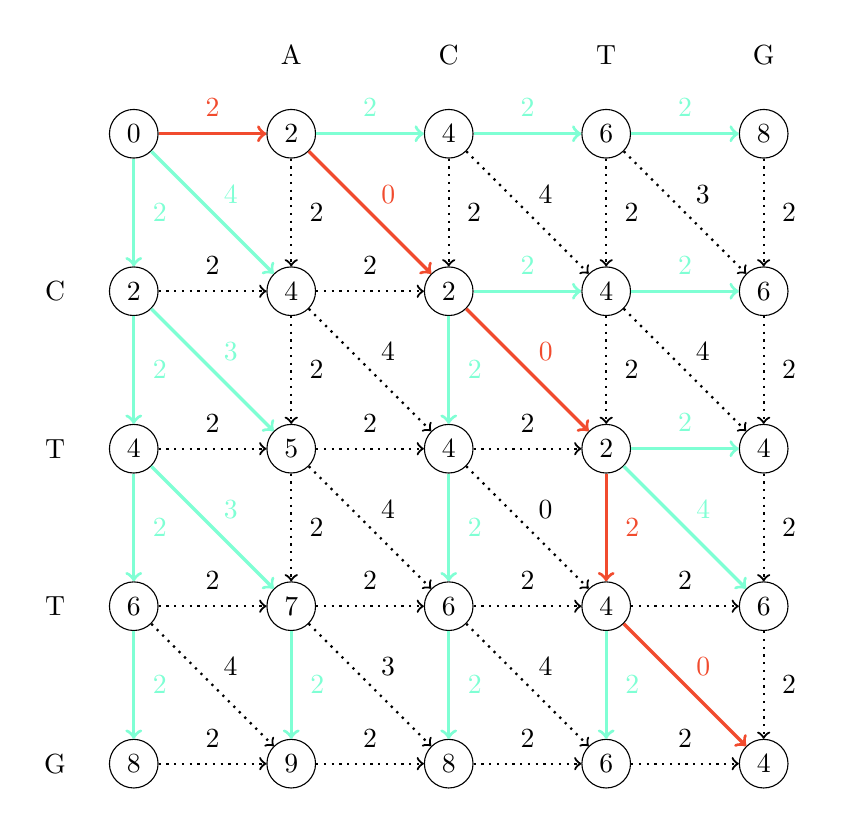
\begin{tikzpicture}[shape=circle,auto]
    \node[draw] (A) at (0,0) {8};
    \node[draw] (B) at (2,0) {9};
    \node[draw] (C) at (4,0) {8};
    \node[draw] (D) at (6,0) {6};
    \node[draw] (E) at (8,0) {4};
    \node[draw] (F) at (0,2) {6};
    \node[draw] (G) at (2,2) {7};
    \node[draw] (H) at (4,2) {6};
    \node[draw] (I) at (6,2) {4};
    \node[draw] (J) at (8,2) {6};
    \node[draw] (K) at (0,4) {4};
    \node[draw] (L) at (2,4) {5};
    \node[draw] (M) at (4,4) {4};
    \node[draw] (N) at (6,4) {2};
    \node[draw] (O) at (8,4) {4};
    \node[draw] (P) at (0,6) {2};
    \node[draw] (Q) at (2,6) {4};
    \node[draw] (R) at (4,6) {2};
    \node[draw] (S) at (6,6) {4};
    \node[draw] (T) at (8,6) {6};
    \node[draw] (U) at (0,8) {0};
    \node[draw] (V) at (2,8) {2};
    \node[draw] (W) at (4,8) {4};
    \node[draw] (X) at (6,8) {6};
    \node[draw] (Y) at (8,8) {8};
    
    \draw (2,9) node{A};
    \draw (4,9) node{C};
    \draw (6,9) node{T};
    \draw (8,9) node{G};
    \draw (-1,0) node{G};
    \draw (-1,2) node{T};
    \draw (-1,4) node{T};
    \draw (-1,6) node{C};

    \draw[thick] (A) edge[dotted, ->] node {2} (B);
    \draw[thick] (B) edge[dotted, ->] node {2} (C);
    \draw[thick] (C) edge[dotted, ->] node {2} (D);
    \draw[thick] (D) edge[dotted, ->] node {2} (E);
    \draw[thick] (F) edge[dotted, ->] node {2} (G);
    \draw[thick] (G) edge[dotted, ->] node {2} (H);
    \draw[thick] (H) edge[dotted, ->] node {2} (I);
    \draw[thick] (I) edge[dotted, ->] node {2} (J);
    \draw[thick] (K) edge[dotted, ->] node {2} (L);
    \draw[thick] (L) edge[dotted, ->] node {2} (M);
    \draw[thick] (M) edge[dotted, ->] node {2} (N);
    \draw[very thick] (N) edge[Aquamarine, ->] node {2} (O);
    \draw[thick] (P) edge[dotted, ->] node {2} (Q);
    \draw[thick] (Q) edge[dotted, ->] node {2} (R);
    \draw[very thick] (R) edge[Aquamarine, ->] node {2} (S);
    \draw[very thick] (S) edge[Aquamarine, ->] node {2} (T);
    \draw[very thick] (U) edge[RedOrange, ->] node {2} (V);
    \draw[very thick] (V) edge[Aquamarine, ->] node {2} (W);
    \draw[very thick] (W) edge[Aquamarine, ->] node {2} (X);
    \draw[very thick] (X) edge[Aquamarine, ->] node {2} (Y);
    \draw[very thick] (F) edge[Aquamarine, ->] node {2} (A);
    \draw[very thick] (G) edge[Aquamarine, ->] node {2} (B);
    \draw[very thick] (H) edge[Aquamarine, ->] node {2} (C);
    \draw[very thick] (I) edge[Aquamarine, ->] node {2} (D);
    \draw[thick] (J) edge[dotted, ->] node {2} (E);
    \draw[very thick] (K) edge[Aquamarine, ->] node {2} (F);
    \draw[thick] (L) edge[dotted, ->] node {2} (G);
    \draw[very thick] (M) edge[Aquamarine, ->] node {2} (H);
    \draw[very thick] (N) edge[RedOrange, ->] node {2} (I);
    \draw[thick] (O) edge[dotted, ->] node {2} (J);
    \draw[very thick] (P) edge[Aquamarine, ->] node {2} (K);
    \draw[thick] (Q) edge[dotted, ->] node {2} (L);
    \draw[very thick] (R) edge[Aquamarine, ->] node {2} (M);
    \draw[thick] (S) edge[dotted, ->] node {2} (N);
    \draw[thick] (T) edge[dotted, ->] node {2} (O);
    \draw[very thick] (U) edge[Aquamarine, ->] node {2} (P);
    \draw[thick] (V) edge[dotted, ->] node {2} (Q);
    \draw[thick] (W) edge[dotted, ->] node {2} (R);
    \draw[thick] (X) edge[dotted, ->] node {2} (S);
    \draw[thick] (Y) edge[dotted, ->] node {2} (T);
    \draw[thick] (F) edge[dotted, ->] node {4} (B);
    \draw[thick] (G) edge[dotted, ->] node {3} (C);
    \draw[thick] (H) edge[dotted, ->] node {4} (D);
    \draw[very thick] (I) edge[RedOrange, ->] node {0} (E);
    \draw[very thick] (K) edge[Aquamarine, ->] node {3} (G);
    \draw[thick] (L) edge[dotted, ->] node {4} (H);
    \draw[thick] (M) edge[dotted, ->] node {0} (I);
    \draw[very thick] (N) edge[Aquamarine, ->] node {4} (J);
    \draw[very thick] (P) edge[Aquamarine, ->] node {3} (L);
    \draw[thick] (Q) edge[dotted, ->] node {4} (M);
    \draw[very thick] (R) edge[RedOrange, ->] node {0} (N);
    \draw[thick] (S) edge[dotted, ->] node {4} (O);
    \draw[very thick] (U) edge[Aquamarine, ->] node {4} (Q);
    \draw[very thick] (V) edge[RedOrange, ->] node {0} (R);
    \draw[thick] (W) edge[dotted, ->] node {4} (S);
    \draw[thick] (X) edge[dotted, ->] node {3} (T);
\end{tikzpicture}
\end{figure*}
%%% Local Variables:
%%% mode: latex
%%% TeX-master: "../rapport"
%%% End:


L'alignement optimal correspondant est donc :
\begin{table*}[h]
  \centering
  \begin{tabular}{c|ccccc}
    \hline
    --&A&C&T&--&G\\
    --&--&C&T&T&G\\
    \hline
  \end{tabular}
\end{table*}

\paragraph{Question 2.4}
La complexit\'e spatiale ne varie pas de celle propos\'ee par
l'algorithme de la partie 1, soit $\Theta(nm)$, l'algorithme de
\emph{Dijkstra} nous donne une arborescence des chemins de co\^uts
minimum en $O(nm\log(nm))$ pour notre probl\`eme ($N=nm$ et
$M=(n-1)(m-1)+n(m-1)+m(n-1)$ avec les notations de la question 2.3),
soit une moins bonne complexit\'e temporelle qu'\`a la partie 1.

\paragraph{Remarque}
On aurais tr\`es bien pu utiliser l'agorithme de \emph{Bellman} vu que
le graphe est sans circuits. Ainsi on aurait une compl\'exit\'e
temporelle en $O(nm)$ pour notre probl\`eme ($(N+M)$ pour un graphe
\`a $N$ sommets et $M$ arcs). La complexit\'e temporelle est
pr\'ef\'erable \`a celle de l'algorithme de Dijkstra, cependant c'est
la m\^eme complexit\'e qu'\`a la partie 1.
%%% Local Variables:
%%% mode: latex
%%% TeX-master: "rapport"
%%% End:
